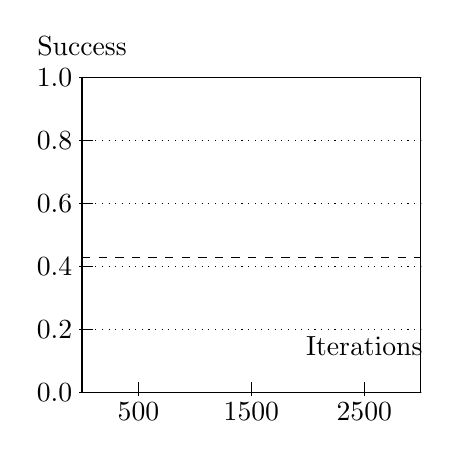
\begin{tikzpicture}[x=0.00143cm,y=4cm]
    % Draw the axes and grid lines
    \draw[-] (0,0) -- (0,1) -- (3000,1) -- (3000,0) -- cycle; 
    \draw[-,thin, dotted, ystep=0.2, xstep=3000] (0,0) grid (3000,1);
    \foreach \x in {500, 1500, 2500}  \draw [-,xshift=0](\x,4pt) -- (\x,-1pt);
    \foreach \y in {0.0,0.2,0.4,0.6,0.8,1.0}  \draw [-,yshift=0](4pt,\y) -- (-1pt,\y);
    \foreach \x/\xtext in {500/500, 1500/1500, 2500/2500} \node at (\x,0) [below] {$\xtext$};
    \foreach \y/\ytext in {0.0,0.2,0.4,0.6,0.8,1.0}  \node at (0,\y) [left] {$\ytext$};
    \node at (0,1.1) {Success};
    \node at (2500,0.15) {Iterations};
    \draw[-] plot[mark=x,mark size=4,mark options={color=black}] 
			file {data/test05v3gm.CP.tikzdata};
    \draw[-] plot[mark=o,mark size=2,mark options={color=black}] 
			file {data/test05v3gm.SP.tikzdata};
    % Also draw the expected convergence: 0.9^8 actions=0.43046
    \draw[dashed,-,yshift=0](0,0.43046) -- (3000,0.43046);

\end{tikzpicture}
